\section{Results} \label{sec:resultsexp}

\subsection{Fillers}

The scores given to the filler sentences help establish baseline values for the extreme points of acceptability. The grammatical fillers received a mean score of 2.08 (\textit{SD} = 1.66) while the ungrammatical fillers received a mean score of $-$1.99 (\textit{SD} = 1.41). However, as a measure of central tendency, median is more suitable for finding the actual centre of ordinal data. In this respect, the medians of both the grammatical and ungrammatical fillers give us the extreme points of the scale, which are 3 and $-$3, respectively. Further descriptive statistics of the fillers can be seen in Table \ref{tab:filler_descriptive}.

\begin{table}[!h]
	\centering
	\begin{tabular}{lrrrrrr}
		\textbf{Filler Type} & \textbf{N} & \textbf{Mean} & \textbf{SD} & \textbf{Min} & \textbf{Max} & \textbf{Median} \\ 
		\hline \hline
		Grammatical & 528 & 2.08 & 1.66 & $-$3 & 3 & 3\\ 
		Ungrammatical & 528 & $-$1.99 & 1.41 & $-$3 & 3 & $-$3 \\ 
		\hline
		\hline
	\end{tabular}
	\caption{Descriptive statistics of the filler sentences}
	\label{tab:filler_descriptive}
\end{table}

\subsection{Coordination of unlike categories}
\subsubsection{Descriptive statistics}

Consistent with expectations, the LCAT-LF condition, representing the standard coordination type in Turkish, achieved the highest average score of 2.45 (\textit{SD} = 1.10, \textit{Mdn} = 3). Its unlike counterpart, UCAT-LF, where conjuncts differed in their categories but matched in their functions, was rated slightly less acceptable but still positive with a mean score of 1.88 (\textit{SD} = 1.53, \textit{Mdn} = 2.5). However, the participants gave poor ratings to the two conditions where the conjuncts had mismatching functions. While LCAT-UF received a mean score of $-$0.80 (\textit{SD} = 1.91, \textit{Mdn} = $-$1), UCAT-UF was rated as the least acceptable coordination type with an average score of $-$0.84 (\textit{SD} = 1.94, \textit{Mdn} = $-$1). Nevertheless, we cannot regard these two conditions as outright unacceptable when we compare their mean scores with the mean score of fully ungrammatical filler sentences, which should be considered as the baseline value for extreme unacceptability. The descriptive statistics of unlike category coordination part of the experiment can be observed in the following table.

\begin{table}[ht]
	\centering
	\begin{tabular}{lrrrrrr}
		\textbf{Coordination type} & \textbf{N} & \textbf{Mean} & \textbf{SD} & \textbf{Min} & \textbf{Max} & \textbf{Median} \\ 
		\hline \hline
		LCAT-LF & 144 & 2.45 & 1.10 &  $-$3 &   3 & 3.00  \\
		UCAT-LF & 144 & 1.88 & 1.53 &  $-$3 &   3 & 2.50  \\ 
		LCAT-UF & 144 & $-$0.80 & 1.91 &  $-$3 &   3 & $-$1.00  \\ 
		UCAT-UF & 144 & $-$0.84 & 1.94 &  $-$3 &   3 & $-$1.00  \\ 
		\hline
		\hline
	\end{tabular}
	\caption{Descriptive statistics of the unlike category coordination experiment} 
\end{table}

As can be seen in the boxplot in Figure \ref{fig:catboxplot}, the participants seem to be in strong agreement when it comes to the high acceptability of LCAT-LF as the IQR box is encapsulated between the scores of 2 and 3 with a relatively short lower whisker length. Likewise, the distribution of scores given to UCAT-LF sentences also follows a clear left-skewed distribution towards the positive end of the scale, although now the IQR range is slightly extended. The participants seem to be in relative disagreement about the acceptability of LCAT-UF and UCAT-UF conditions as scores given to these conditions explore the full range of the Likert scale. Ultimately, however, both LCAT-UF and UCAT-UF received negative mean and median scores that were significantly lower than their counterparts. 

\begin{figure}[!h]
	\centering
	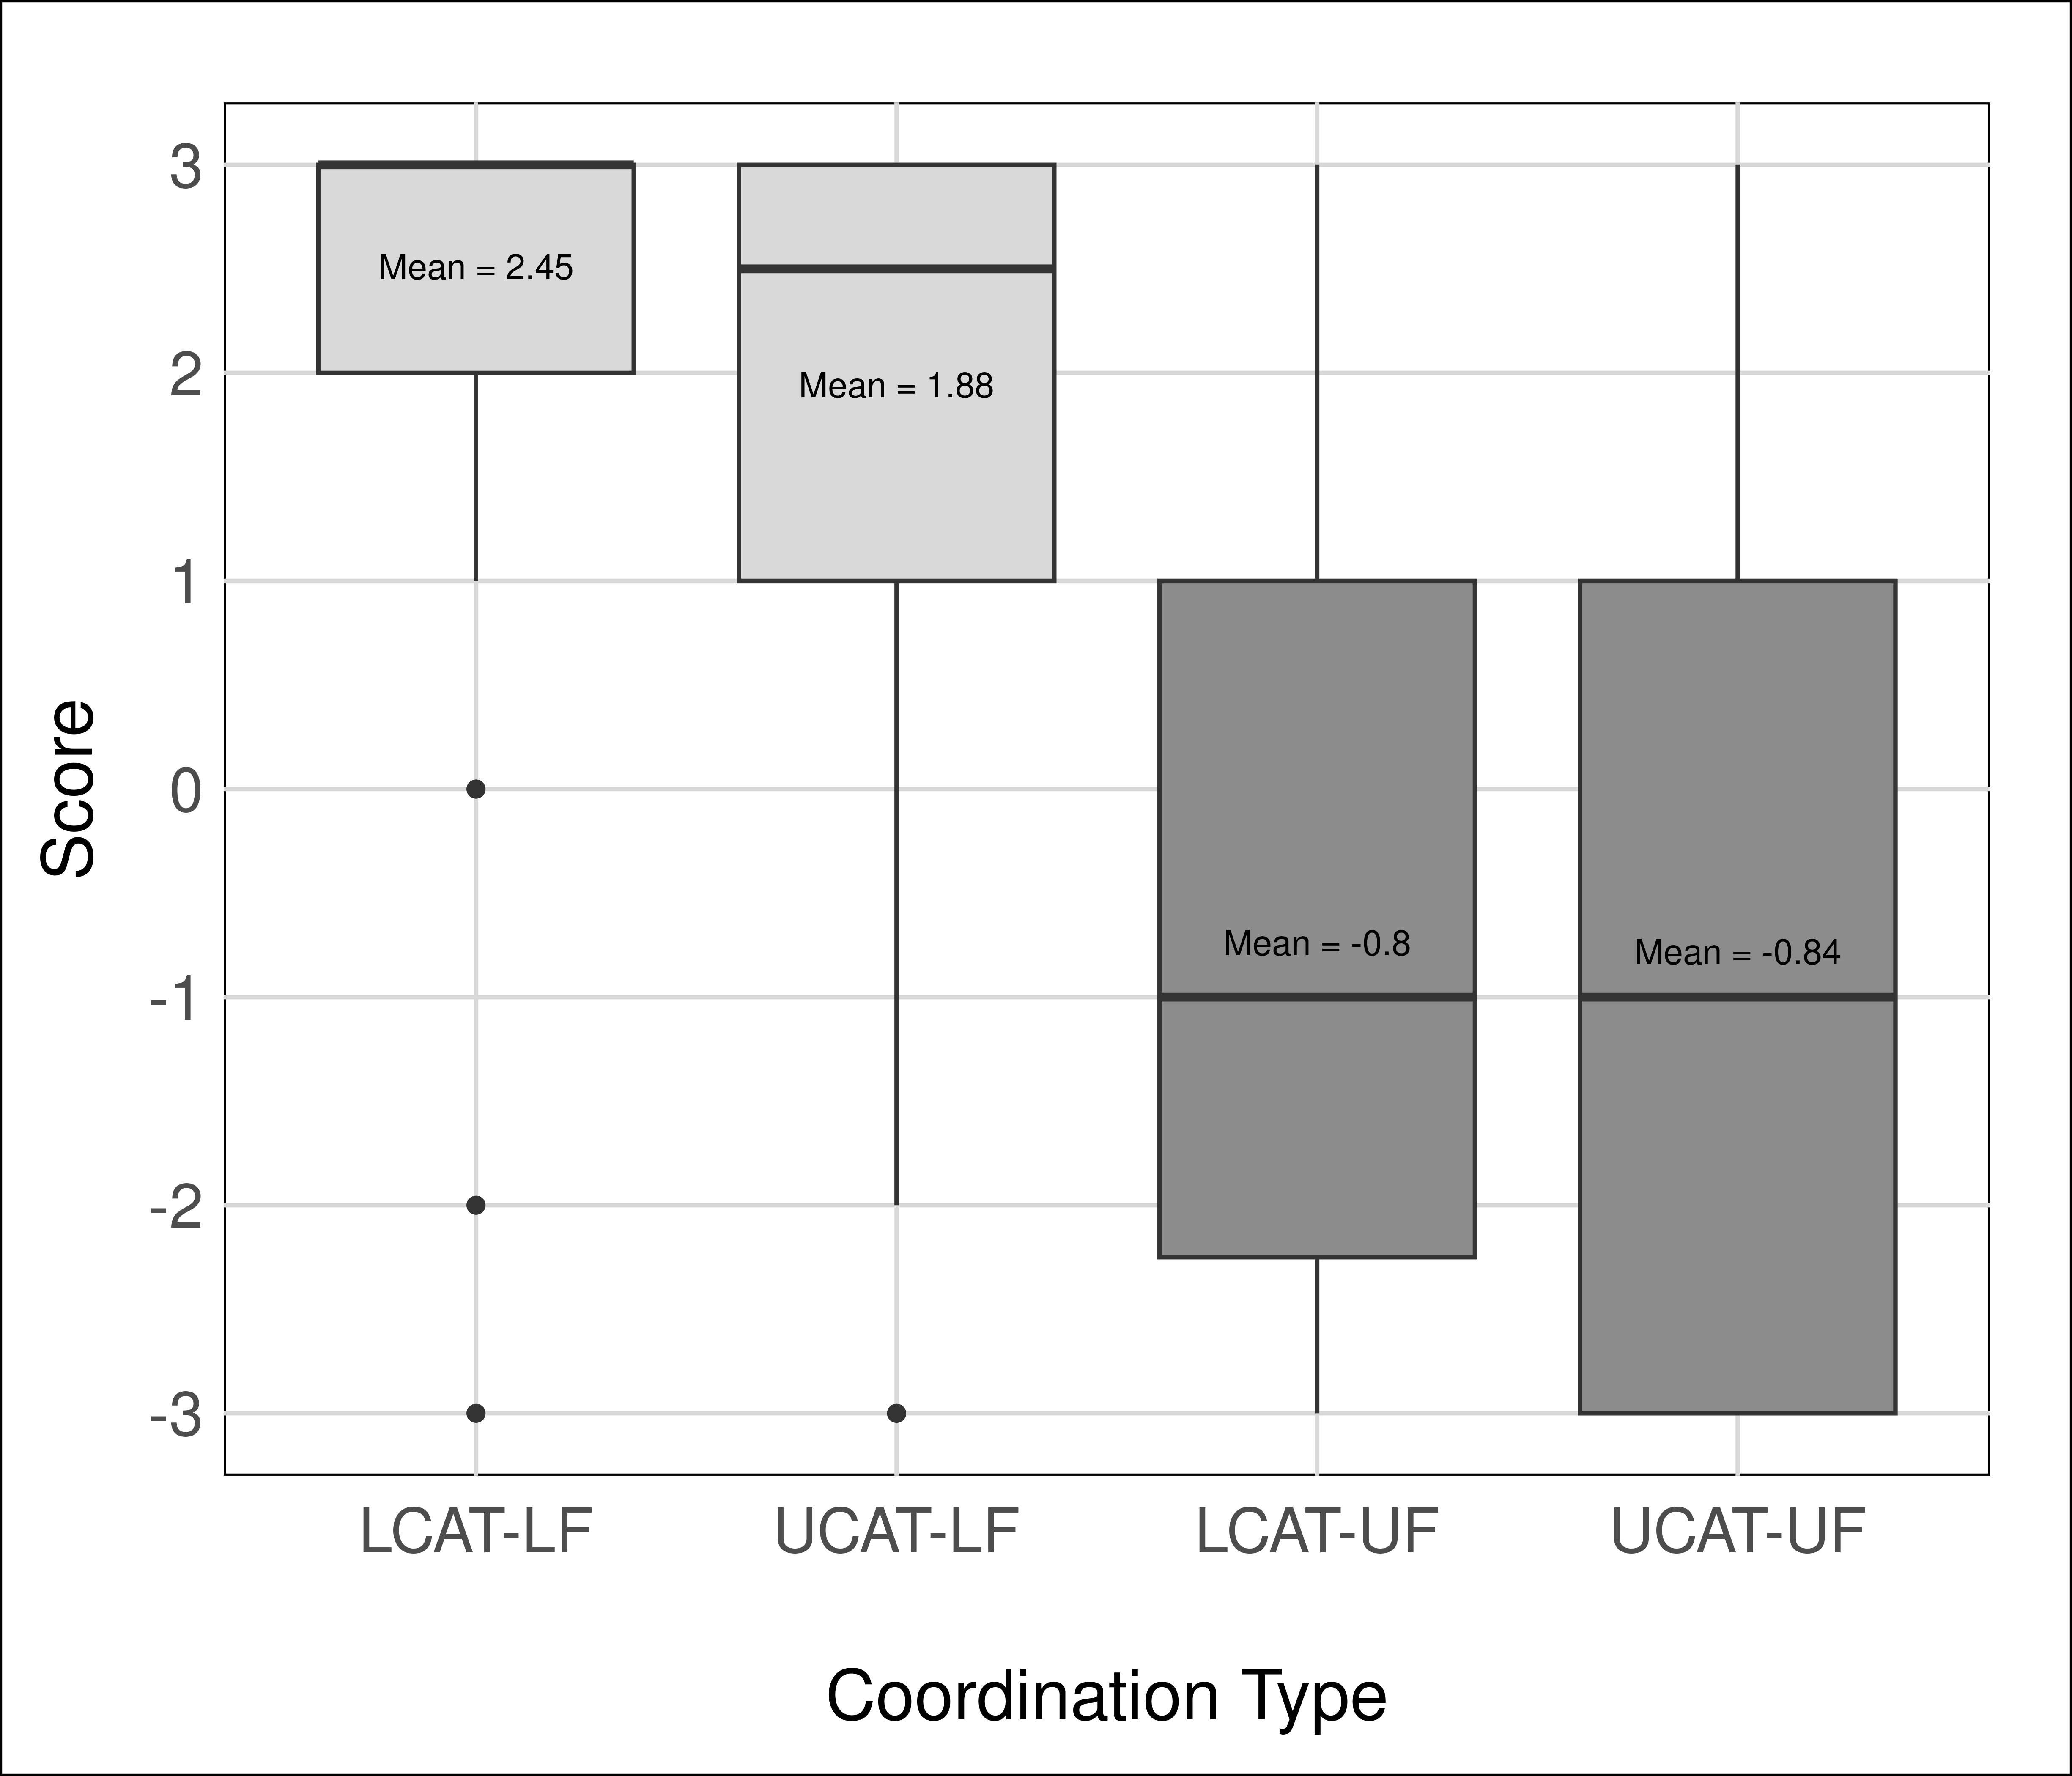
\includegraphics[width=0.88\linewidth]{images/updated_experiment/catboxplot.png}
	\caption{Boxplot for unlike category coordination experiment}
	\label{fig:catboxplot}
\end{figure}

\subsubsection{Inferential statistics}

Before fitting the linear mixed-effects models, several relevant comparisons between different pairs of conditions were carried out. A Wilcoxon signed-rank test was conducted to compare the scores for the LCAT-LF and UCAT-LF conditions. The test revealed a significant difference between the two conditions, with a test statistic (\textit{V}) of 2563 (\textit{p} < 0.001). This finding is in conflict with the part of the hypothesis that there should be no significant difference in acceptability so long as the conjuncts match in their functions. However, the same test demonstrated that UCAT-LF was also significantly different from both LCAT-UF (\textit{V} = 7735, \textit{p} < 0.001) and UCAT-UF (\textit{V} = 7394, \textit{p} < 0.001). 

Three distinct linear models were fitted to unlike category coordination data. In the first model, the distinct coordination configurations (i.e., LCAT-LF, UCAT-LF, LCAT-UF, UCAT-UF) were encoded as the levels of one independent variable called ``conditions.'' While this independent variable was specified as the fixed effect, IDs of the participants and token set indices were encoded as random effects. The exact R code used to fit the model can be seen in Figure \ref{fig:R_catmodelbasic}. Since the default optimiser of the `lmer()' function, the ``nloptwrap'' algorithm, failed to produce a fully convergent model, the ``bobyqa'' algorithm was used.

\begin{figure}[!h]
	\lstset{
		language=R,
		escapechar=@,
		basicstyle=\small\ttfamily,
		columns=fullflexible,
		keepspaces=true,
		keywordstyle=\color{black}\bfseries
	}
	\begin{lstlisting}
		control <- lmerControl(optimizer = "bobyqa")
		
		model_cat_1factor <- lmer(rating ~ condition +
		(1 + condition|participant_ID) +
		(1 + condition|tokenset),
		data = lm_cat_1factor,
		control = control)\end{lstlisting}
	\caption{R code for Model I of unlike category coordination experiment data}
	\label{fig:R_catmodelbasic}
\end{figure}


The relevant specifications of the first model (including some random effect statistics) are summarized in Figure \ref{tab:lmbasic}. 


\begin{table}[!h]
	\centering
	\begin{tabular}{llrr}
		\hline
		\hline
		\multicolumn{1}{c}{\textbf{}}        & \multicolumn{3}{c}{\textbf{acceptability}}                                            \\
		\multicolumn{1}{c}{\textit{Predictors}}       & \multicolumn{1}{c}{\textit{Estimates}} & \multicolumn{1}{c}{\textit{CI}} & \multicolumn{1}{c}{\textit{p}} \\ \hline
		(Intercept)                          & \multicolumn{1}{r}{2.45}      & 2.20 - 2.71            & \textbf{\textless{} 0.001}    \\
		condition {[}UCAT-LF{]}              & \multicolumn{1}{r}{--0.58}   &--1.04 - --0.13          & \textbf{0.012}                 \\
		condition {[}LCAT-UF{]}              & \multicolumn{1}{r}{--3.25}     & --3.75 - --2.75          & \textbf{\textless{} 0.001}    \\
		condition {[}UCAT-UF{]}              & \multicolumn{1}{r}{--3.29}     & --3.82 - --2.76          & \textbf{\textless{} 0.001}     \\
		\multicolumn{4}{l}{\textbf{Random Effects}}                                                                                    \\
		$\sigma$2                                   & \multicolumn{3}{l}{1.59}                                                       \\
		$\tau$00 participant\_ID                  & \multicolumn{3}{l}{0.04}                                                       \\
		$\tau$00 token\_set                       & \multicolumn{3}{l}{0.06}                                                       \\
		N participant\_ID                        & \multicolumn{3}{l}{48}                                                         \\ 
		N token\_set                         & \multicolumn{3}{l}{12}                                                         \\ \hline
		Observations                         & \multicolumn{3}{l}{576}                                                        \\
		Marginal R$^{2}$ / Conditional R$^{2}$        & \multicolumn{3}{l}{0.587 / NA}     \\    
		\hline \hline                                       
	\end{tabular}
	\caption{One independent variable model specifications}
	\label{tab:lmbasic}
\end{table}

In the context of a linear mixed effects model, the fixed effects refer to the parameters that are estimated to have a consistent effect on the outcome variable across all levels of the random effects. The respective coefficients of each level of the fixed effect are interpreted as follows:

\begin{itemize}
	\item \textbf{LCAT-LF}: The intercept coefficient of the model, which is 2.45 (\textit{SE} = 0.13, 95\% \textit{CI} [2.20, 2.71], \textit{p} < 0.001), represents the average rating for the LCAT-LF condition. This means that, on average, participants rated the LCAT-LF stimuli 2.45 on the scale. 
	
	\item \textbf{UCAT-LF}: The coefficient for the UCAT-LF condition is $-$0.58 (\textit{SE} = 0.17, 95\% \textit{CI} [--1.04, --0.13], \textit{p} = 0.012), indicating that participants rated the UCAT-LF stimuli slightly lower by 0.58 points, on average, compared to the LCAT-LF stimuli.
	
	\item \textbf{LCAT-UF}: The coefficient for the LCAT-UF condition is $-$3.25 (\textit{SE} = 0.25, 95\% \textit{CI} [--3.75, --2.75], \textit{p} < 0.001), which represents the difference in average scores between LCAT-UF and LCAT-LF when all other predictors are controlled for. The negative coefficient suggests that participants rated the LCAT-UF stimuli 3.25 points lower than the LCAT-LF stimuli, on average. 
	
	
	\item \textbf{UCAT-UF}: Finally, the coefficient for the UCAT-UF condition is $-$3.29 (\textit{SE} = 0.25, 95\% \textit{CI} [--3.82, --2.76], \textit{p} < 0.001), indicating that participants rated the UCAT-UF stimuli 3.29 points lower than the LCAT-LF stimuli, on average. 
\end{itemize}

Table \ref{tab:comparisons} below provides pairwise comparisons of conditions in the first model. Each row represents a specific comparison between two conditions. The ``Estimate'' column displays the estimated difference between the conditions. For example, in the LCAT-LF $\sim$ LCAT-UF comparison, the estimate of 3.2517 suggests that, on average, LCAT-LF condition is estimated to receive a higher score than the LCAT-UF condition. The ``SE'' column shows the standard error of the estimate while ``t-ratio'' column displays the calculated t-ratio for the comparison. The ``p-value'' column indicates the probability of obtaining the observed t-ratio or a more extreme value if the null hypothesis (no difference between the conditions) is true.

From the table, we can observe that the LCAT-LF $\sim$ LCAT-UF and LCAT-LF $\sim$ UCAT-UF comparisons have significant differences, as evinced by the very small p-values (both <0.0001). However, the LCAT-LF $\sim$ UCAT-LF comparison does not attain statistical significance (\textit{p} = 0.1114), suggesting that the difference between these conditions is not statistically significant. Similarly, the LCAT-UF $\sim$ UCAT-UF comparison shows that their negative impact on scores is virtually the same (\textit{p} = 0.9983). Moreover, the LCAT-UF $\sim$ UCAT-LF and UCAT-LF $\sim$ UCAT-UF comparisons both demonstrate significant differences, with p-values less than 0.0001.


\begin{table}[!ht]
	\centering
	\begin{tabular}{lrrrr}
		\textbf{Comparison} & \textbf{Estimate} & \textbf{SE} & \textbf{t-ratio} & \textbf{p-value} \\
		\hline \hline
		LCAT-LF $\sim$ UCAT-LF & 0.5810 & 0.232 & 2.508 & 0.1114 \\
		LCAT-LF $\sim$ LCAT-UF & 3.2517 & 0.256 & 12.682 & <0.0001 \\
		LCAT-LF $\sim$ UCAT-UF & 3.2941 & 0.270 & 12.186 & <0.0001 \\
		UCAT-LF $\sim$ UCAT-UF & 2.7132 & 0.372 & 7.298 & <0.0001 \\
		LCAT-UF $\sim$ UCAT-LF & $-$2.6708 & 0.299 & $-$8.934 & <0.0001 \\
		LCAT-UF $\sim$ UCAT-UF & 0.0424 & 0.258 & 0.164 & 0.9983 \\
		\hline
		\hline
	\end{tabular}
	\caption{Pairwise comparisons of conditions in Model I}
	\label{tab:comparisons}
\end{table}


The second model had two independent variables as fixed effects. These were the binary categorical variables of ``function'' and ``category'' where 1 indicated that conjuncts matched in their grammatical functions or categories, respectively. This model makes it possible to better isolate and estimate the individual impacts of functional and categorical matching between the conjuncts on the acceptability scores of the participants. While Figure \ref{fig:R_catmodel} shows the exact R code to fit the model, Figure \ref{fig:lmcat} lists the exact specifications of the second model. As this model could reach full convergence with the default optimizer algorithm, no alterations were introduced.

\begin{figure}[!h]
	\lstset{
		language=R,
		escapechar=@,
		basicstyle=\small\ttfamily,
		columns=fullflexible,
		keepspaces=true
	}
	\begin{lstlisting}
		model_cat <- lmer(rating ~ 
		function_match + category_match +
		(function_match + category_match | participant_ID) +
		(function_match + category_match | tokenset),
		data = lm_cat)\end{lstlisting}
	\caption{R code for Model II of unlike category coordination experiment data}
	\label{fig:R_catmodel}
\end{figure}

\begin{table}[!h]
	\centering
	\begin{tabular}{llrr}
		& \multicolumn{3}{c}{\textbf{acceptability}}                   \\
		\textit{Predictors} & \textit{Estimates}        & \multicolumn{1}{l}{\textit{CI}} & \multicolumn{1}{l}{\textit{p}} \\ \hline
		(Intercept)                  & \multicolumn{1}{r}{2.32}  & {2.00} - {2.65}   & \textless{}0.001 \\
		function mismatch   & \multicolumn{1}{r}{--2.99} & {--3.46} - {--2.51}                   & \textless{}0.001               \\
		category mismatch            & \multicolumn{1}{r}{--0.31} & --0.59 - --0.03 & 0.029            \\
		\multicolumn{4}{l}{\textbf{Random Effects}}                                                 \\
		$\sigma^{2}$                           & \multicolumn{3}{l}{1.79}                                     \\
		$\tau$00 participant\_ID          & \multicolumn{3}{l}{0.16}                                     \\
		$\tau$00 token\_set               & \multicolumn{3}{l}{0.18}                                     \\
		N participant\_ID                        & \multicolumn{3}{l}{48}                                                         \\ 
		N token\_set                 & \multicolumn{3}{l}{12}                                       \\ \hline
		Observations                 & \multicolumn{3}{l}{576}                                      \\
		Marginal R$^{2}$ / Conditional R$^{2}$ & \multicolumn{3}{l}{0.558 / NA}  \\ \hline \hline                            
	\end{tabular}
	\caption{Two independent variables model specifications}
	\label{fig:lmcat}
\end{table}


The intercept of the second model, which represents the average score when both functions and categories of the conjuncts match, was found to be 2.32 (\textit{SE} = 0.16, 95\% \textit{CI} [2.00, 2.65], \textit{p} < 0.001). The estimated coefficient for function mismatch was $-$2.99 (\textit{SE} = 0.23, 95\% \textit{CI} [$-$3.46, $-$2.51], \textit{p} < 0.001), indicating that when the functions of the conjuncts do not match, the average rating is expected to decrease by 2.99. The coefficient for category mismatch was $-$0.31 (\textit{SE} = 0.14, 95\% \textit{CI} [$-$0.59, $-$0.03], \textit{p} = 0.029), suggesting that the average rating is expected to decrease by 0.31 when the conjuncts have different syntactic categories.

The results of this model suggest that both function mismatch and category mismatch have a significant impact on the acceptability ratings. When the functions of the conjuncts do not match, however, the acceptability scores dramatically decrease, while a mismatch in syntactic categories leads to only a slight decrease in scores.

Note that the intercept of the second model refers to the score of the condition LCAT-LF. It is, however, different from the intercept of the first model, which corresponds to the same variable. This stems from the fact that the second model does not take into account the interaction between the two fixed effects. For this reason, a third model was also fit to the data to account for the interaction between the fixed effects of function mismatch and category mismatch as well. The Figure \ref{fig:R_catmodel2} demonstrates the exact R code used to fit the model. The Table \ref{tab:catmodel3}, on the other hand, provides the estimates, confidence intervals, and p-values for each predictor in this model. 


\begin{figure}[!h]
	\lstset{
		language=R,
		escapechar=@,
		basicstyle=\small\ttfamily,
		columns=fullflexible,
		keepspaces=true
	}
	\begin{lstlisting}
		model_cat_interaction <- lmer(rating ~ 
		function_match * category_match +
		(function_match + category_match | participant_ID) +
		(function_match + category_match | tokenset),
		data = lm_cat)\end{lstlisting}
	\caption{R code for Model III of unlike category coordination experiment data}
	\label{fig:R_catmodel2}
\end{figure}


\begin{table}[!h]
	\centering
	\begin{tabular}{llrr}
		\hline \hline
		\multicolumn{1}{c}{\textbf{}}         & \multicolumn{3}{c}{\textbf{acceptability}}                          \\
		\multicolumn{1}{c}{\textit{Predictors}} & \multicolumn{1}{c}{\textit{Estimates}} & \multicolumn{1}{c}{\textit{CI}} & \multicolumn{1}{c}{p} \\ \hline
		(Intercept)                           & \multicolumn{1}{r}{2.45}  & 2.11 – 2.80   & \textless{}0.001 \\
		function mismatch                     & \multicolumn{1}{r}{-3.26} & -3.78 – -2.73 & \textless{}0.001 \\
		category mismatch                     & \multicolumn{1}{r}{-0.58} & -0.94 – -0.22 & 0.002            \\
		function mismatch × category mismatch & \multicolumn{1}{r}{0.54}  & 0.10 – 0.98   & 0.015            \\
		\multicolumn{4}{l}{\textbf{Random Effects}}                                                          \\
		$\sigma$2                                    & \multicolumn{3}{l}{1.77}                                     \\
		$\tau$00 participant\_ID                   & \multicolumn{3}{l}{0.16}                                     \\
		$\tau$00 token\_set                        & \multicolumn{3}{l}{0.18}                                     \\
		N participant\_ID                        & \multicolumn{3}{l}{48}                                                         \\
		N token\_set                          & \multicolumn{3}{l}{12}                                       \\ \hline
		Observations                          & \multicolumn{3}{l}{576}                                      \\
		Marginal R2 / Conditional R2          & \multicolumn{3}{l}{0.563 / NA} \\ \hline \hline                              
	\end{tabular}
	\caption{Two independent variables + interaction model specifications}
	\label{tab:catmodel3}
\end{table}
The intercept of the third model (see Table \ref{tab:catmodel3}) indicates that the expected acceptability rating is 2.45 when conjuncts match both in their functions and categories (\textit{SE} = 0.17, 95\% \textit{CI} [2.11, 2.80], \textit{p} < 0.001). The estimate for the function mismatch variable is $-$3.26 (\textit{SE} = 0.26, 95\% \textit{CI} [$-$3.78, $-$2.73], \textit{p} < 0.001), indicating that a mismatch of functions is associated with an (average) decrease of 3.26 in the acceptability rating when other predictors are held constant. The estimate for the category mismatch is $-$0.58 (\textit{SE} = 0.18, 95\% \textit{CI} [$-$0.94, $-$0.22], \textit{p} = 0.002). That is, mismatching categories of conjuncts is associated with a decrease of 0.58 in the acceptability rating. 

The interaction predictor, function mismatch $\times$ category mismatch, has an estimate of 0.54 (\textit{SE} = 0.22, 95\% \textit{CI} [0.10, 0.98], \textit{p} = 0.015). This means that, on average, when both the functions and the categories of conjuncts mismatch, their cumulative negative effect on the acceptability rating becomes less severe. To calculate the combined effect, we would sum the estimates of the individual main effects (-3.26 for function mismatch and -0.58 for category mismatch) along with the estimate for the interaction term, which is 0.54.


\subsubsection{Discussion}

The results obtained from the three models demonstrate that a functional match between the conjuncts is a crucial factor in the acceptability rate of a coordinate structure. In the first model, the conditions where the conjuncts have different functions (i.e., LCAT-UF and UCAT-UF) have large negative impacts on the acceptability ratings. The predictors of the second model indicates that the functional match between conjuncts has the biggest impact on the acceptability ratings with a coefficient estimate of $-$2.99. In the third model, the negative impact of mismatching functions becomes more pronounced at an estimated coefficient of $-$3.26 when the model accounted for the interaction effects between the predictors.

With the exception of the pairwise comparisons in Model I (see Table \ref{tab:comparisons}), all the analyses show that there is a significant difference between LCAT-LF and UCAT-LF in their acceptability rates. Thus, a categorical incongruity between the conjuncts seems to have a statistically significant impact on the acceptability rate. This impact, however, is not substantial as can be seen from the relevant coefficients of categorical predictors in the models. Furthermore, UCAT-LF is by no means an utterly unacceptable construction as it received a mean score of 1.88 and a median of 2.5 compared to the negative mean scores of LCAT-UF and UCAT-UF conditions. 

Based on the results, two distinct conclusions can be drawn. First, we can challenge the original hypothesis and propose a more flexible version of it, implying that the mismatch between syntactic categories or cases could potentially exert a significant influence on acceptability. Alternatively, we can seek to retain the original hypothesis by considering the impact of frequency factors on acceptability. Within the context of the present findings, LCAT-LF, which is the standard type of coordination in Turkish, is undeniably much more frequent in Turkish corpora than UCAT-LF. In experimental syntax literature, there is a substantial body of evidence indicating that structures with low frequencies tend to receive lower acceptability ratings when compared to high-frequency structures, assuming both structures are grammatical \citep{Bresnan2007, Divjak2016, Francis2021}. Therefore, a minor disparity in favor of the LCAT-LF condition is expected.

As a result, the present thesis leans towards the latter conclusion, thereby upholding the original hypothesis. This stance essentially asserts that the slight variation in acceptability ratings between the conditions could be attributed to the frequency difference between the LCAT-LF and UCAT-LF conditions.

\subsection{Coordination of unlike cases}
\subsubsection{Descriptive statistics}

As demonstrated in Table \ref{tab:unlikecase_descriptive}, the mean rating for LCASE-LF coordination type is 2.32, with a standard deviation of 1.38. The median rating is 3, indicating a generally positive evaluation of this coordination type, which is not surprising as this is the standard type of coordination in Turkish. On the other hand, the mean rating for UCASE-LF coordination type is 1.58, with a higher standard deviation of 1.71. The median rating is 2.00, suggesting a positive evaluation of this coordination type, but with more variability than LCASE-LF. Finally, the mean rating for UCASE-UF coordination type is negative at $-$0.37, with the highest standard deviation of 2.04. The median rating is $-$1.00, indicating an overall negative evaluation of this coordination type. 

\begin{table}[ht]
	\centering
	\begin{tabular}{lrrrrrr}
		\textbf{Coordination type} & \textbf{N} & \textbf{Mean} & \textbf{SD} & \textbf{Min} & \textbf{Max} & \textbf{Median}  \\ 
		\hline \hline
		LCASE-LF & 144 &2.32 & 1.38 &  $-$3 &   3 & 3.00  \\ 
		UCASE-LF & 144 &1.58 & 1.71 &  $-$3 &   3 & 2.00  \\ 
		UCASE-UF & 144 &$-$0.37 & 2.04 &  $-$3 &   3 & $-$1.00  \\ 
		\hline \hline
	\end{tabular}
	\caption{Descriptive statistics of unlike case coordination experiment}
	\label{tab:unlikecase_descriptive} 
\end{table}

Participants strongly agree that LCASE-LF is highly acceptable, as can be seen in Figure \ref{fig:lmcase}. The scores of UCASE-LF, however, show more variability as the IQR box is relatively more spread out between the scores of 1 and 3. UCASE-LF, however, still seems to be an acceptable type as the distribution is again considerably left-skewed towards the positive end of the scale. UCASE-UF, on the other hand, seems to be slightly right-skewed towards the negative end of the scale. The variability of UCASE-UF scores, however, is quite high as IQR box is extended between the scores of $-$2 and 1.


\begin{figure}[!h]
	\centering
	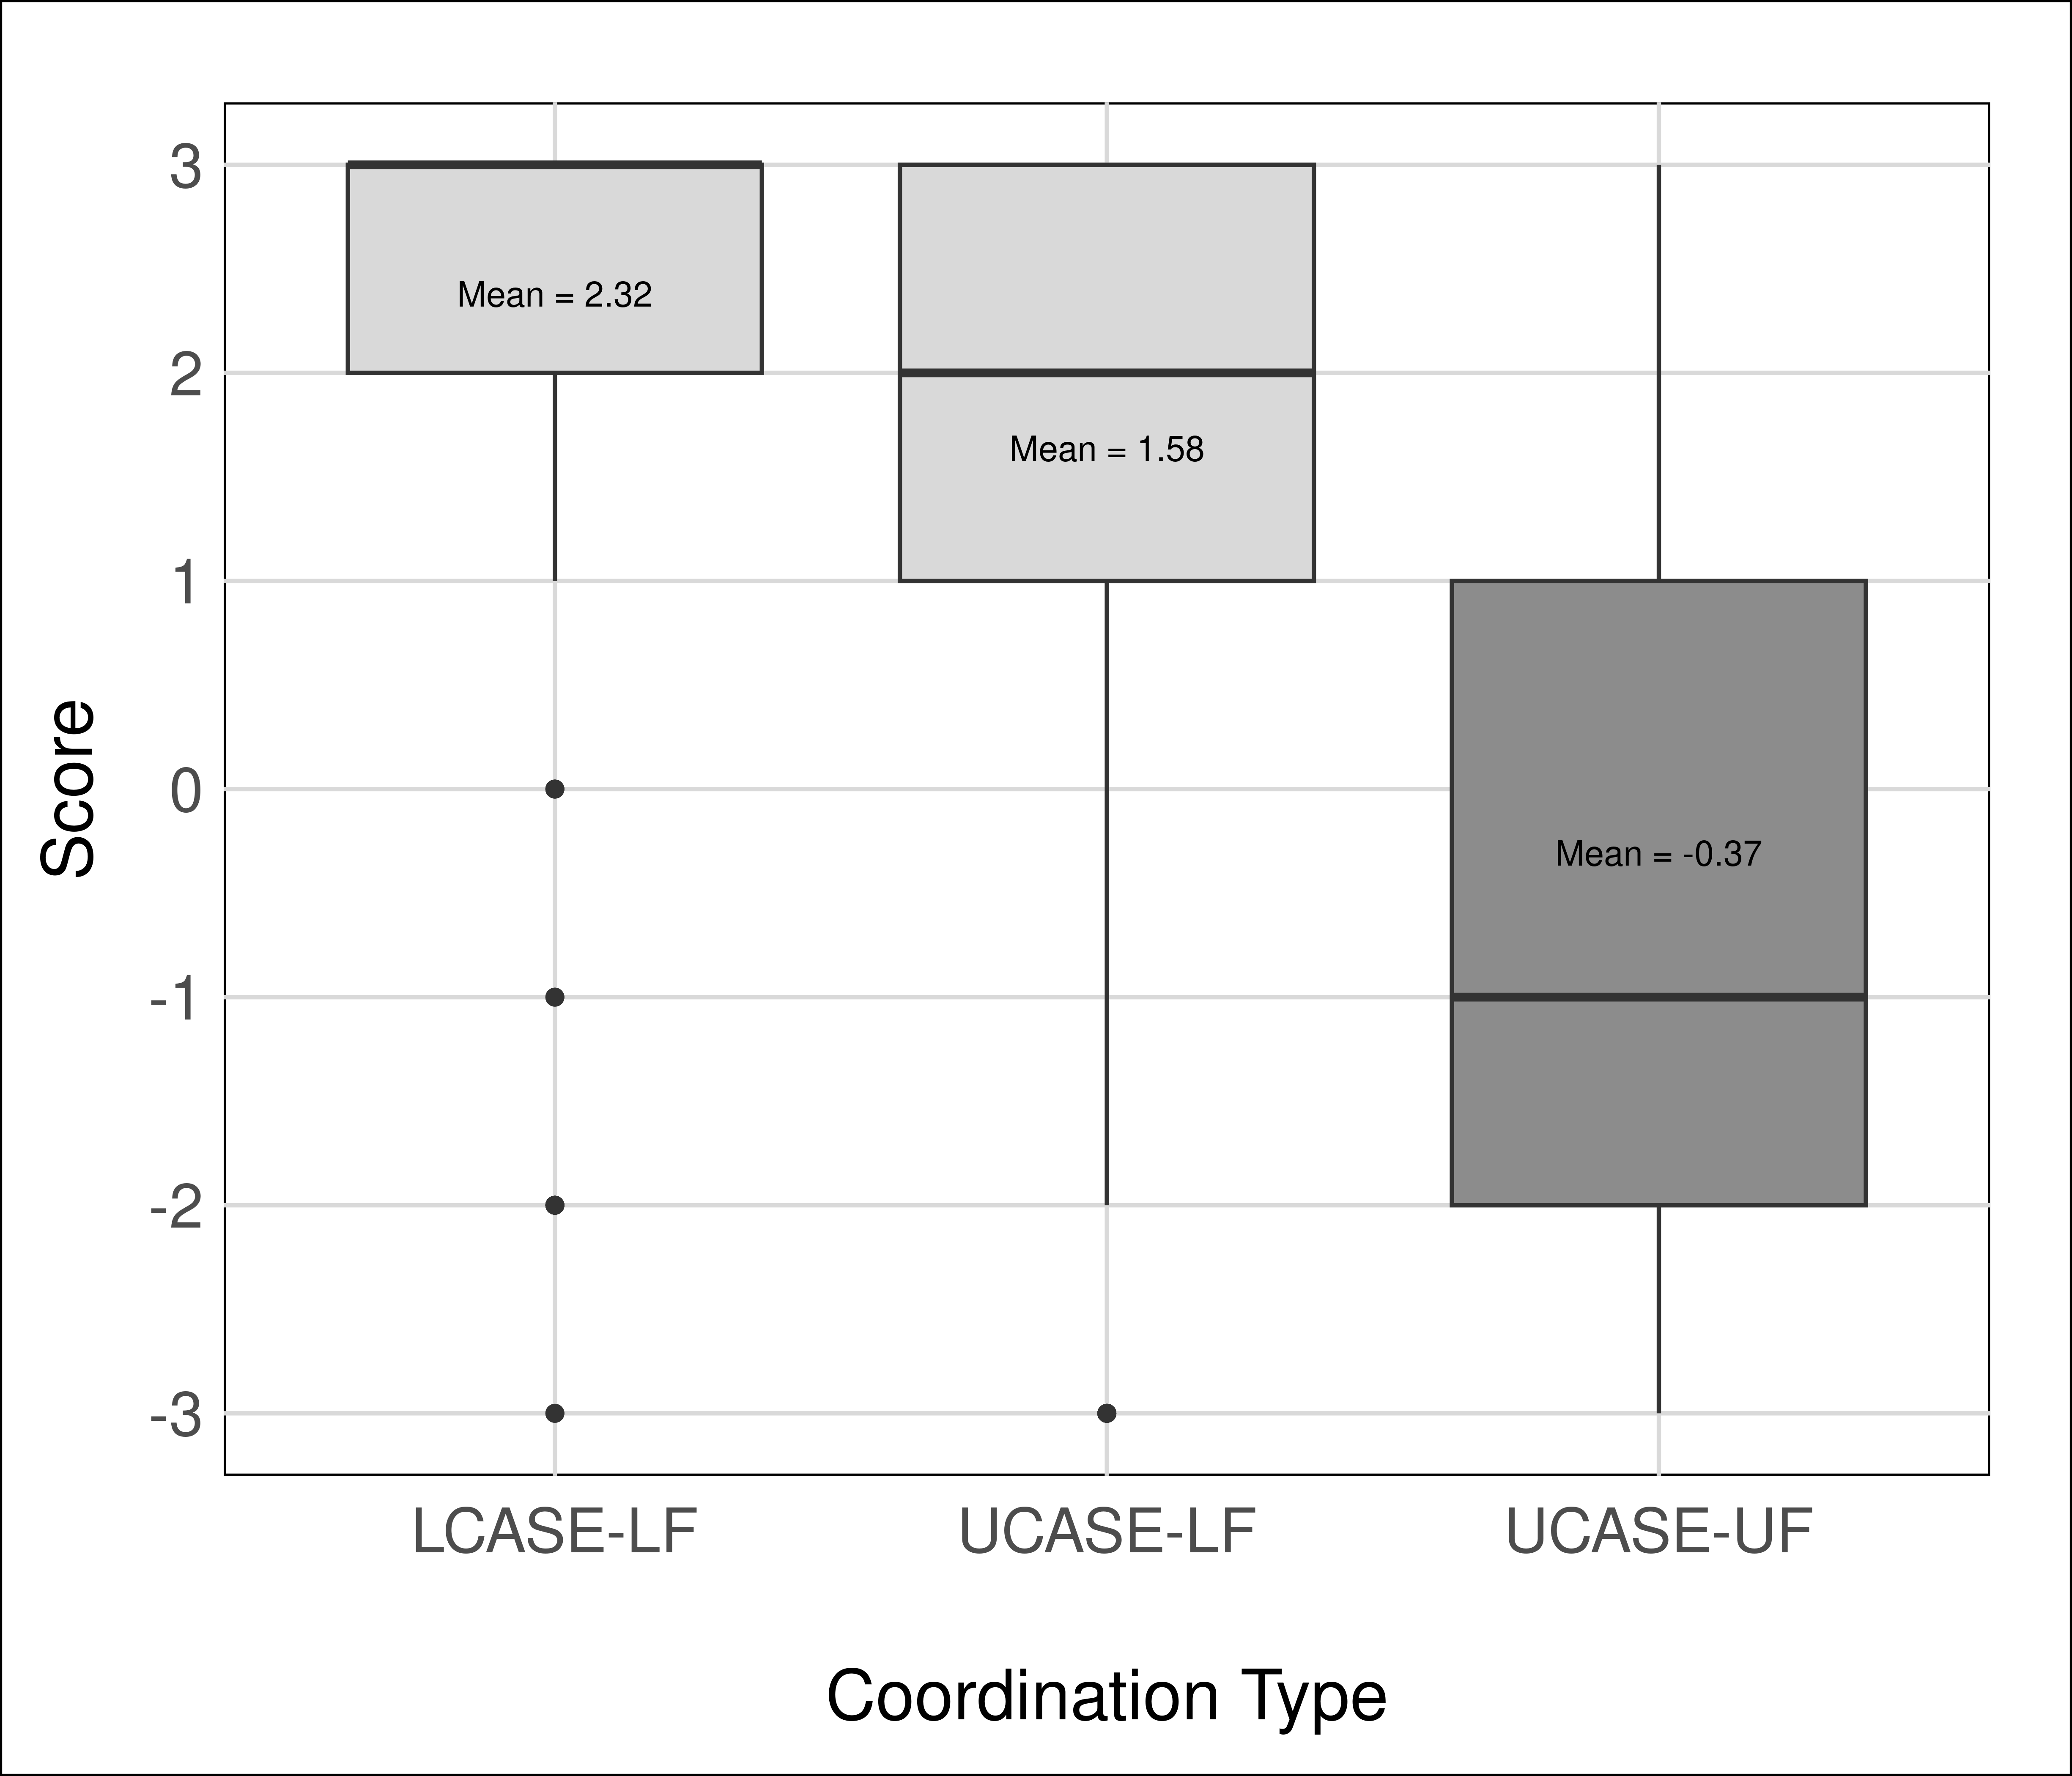
\includegraphics[width=0.88\linewidth]{images/updated_experiment/caseboxplot.png}
	\caption{Boxplot for unlike case coordination experiment}
	\label{fig:lmcase}
\end{figure}


\subsubsection{Inferential Statistics}

Similar to the analyses of unlike category coordination experiment, in addition to fitting a linear mixed-effects model, several Wilcoxon signed-rank tests were conducted to compare relevant pairs of conditions. The difference between LCASE-LF and UCASE-LF was significant (\textit{V} = 2655, \textit{p} < .001), confirming that mismatching cases of conjuncts had a significant negative impact on acceptability. However, the difference between UCASE-LF and UCASE-UF was also significant (\textit{V} = 5859, \textit{p} < .001), suggesting functional incongruity between the conjuncts also had a considerable negative impact on acceptability.

As opposed to the unlike category coordination experiment, only one linear mixed-effects model was fitted to the data as unlike case coordination experiment did not have a proper 2$\times$2 factorial design (see \S \ref{sec:experimentaldesign}). This model is practically the same as the first model used to analyze the unlike category coordination experiment.

This model had one independent variable called ``condition'' encoded as the fixed effect. The distinct types of coordination (i.e., LCASE-LF, UCASE-LF, UCASE-UF) were analyzed as the levels of this variable. The random effects were the same as the previous models: IDs of the participants and the token set indices. Since this model also did not fully converge with the default optimizer algorithm, ``bobyqa'' algorithm had to be manually introduced. The exact code used to fit the model can be seen in Figure \ref{fig:R_casemodel}. The specifications of the fitted model are summarized in Table \ref{tab:lmcase_model}. 

\begin{figure}[!h]
	\lstset{
		language=R,
		escapechar=@,
		basicstyle=\small\ttfamily,
		columns=fullflexible,
		keepspaces=true
	}
	\begin{lstlisting}
		control <- lmerControl(optimizer = "bobyqa")
		
		model_case = lmer(rating ~ condition + 
		(1 + condition|participant_ID) +
		(1 + condition|tokenset), 
		data = lm_case,
		control = control)\end{lstlisting}
	\caption{R code for the model of unlike case coordination experiment data}
	\label{fig:R_casemodel}
\end{figure}


\begin{table}[!h]
	\centering
	\begin{tabular}{llrr}
		\hline \hline
		\multicolumn{1}{c}{\textbf{}} & \multicolumn{3}{c}{\textbf{acceptability}}                          \\
		\multicolumn{1}{c}{\textit{Predictors}} & \multicolumn{1}{c}{\textit{Estimates}} & \multicolumn{1}{c}{\textit{CI}} & \multicolumn{1}{c}{\textit{p}} \\ \hline
		(Intercept)                   & \multicolumn{1}{r}{2.32}  &2.02 -- 2.62   & \textless{}0.001 \\
		condition {[}UCASE-LF{]}        & \multicolumn{1}{r}{-0.75} &-1.15 -- -0.34 & \textless{}0.001 \\
		condition {[}UCASE-UF{]}        & \multicolumn{1}{r}{-2.70} & -3.31 – -2.09 & \textless{}0.001 \\
		\multicolumn{4}{l}{\textbf{Random Effects}}                                                  \\
		$\sigma$2                            & \multicolumn{3}{l}{1.93}                                     \\
		$\tau$00 participant\_ID           & \multicolumn{3}{l}{0.22}                                     \\
		$\tau$00 token\_set                & \multicolumn{3}{l}{0.06}                                     \\
		N token\_set                  & \multicolumn{3}{l}{12}                                       \\ \hline
		Observations                  & \multicolumn{3}{l}{432}                                      \\
		Marginal R2 / Conditional R2  & \multicolumn{3}{l}{0.300 / 0.554}  \\ \hline \hline                      
	\end{tabular}
	\caption{One independent variable case model specficiations}
	\label{tab:lmcase_model}
\end{table}


As revealed by the model, participant scores were significantly affected by the experimental conditions UCASE-LF and UCASE-UF. The intercept, representing the expected score for LCASE-LF, was estimated to be 2.32 (\textit{SE} = 0.15, 95\% \textit{CI} [2.02, 2.62], \textit{p} < 0.001). The scores given to UCASE-LF stimuli were 0.75 points lower (\textit{SE} = 0.20, 95\% \textit{CI} [$-$1.15, $-$0.34], \textit{p} < 0.001) than LCASE-LF condition, on average. UCASE-UF stimuli received 2.70 points lower scores (\textit{SE} = 0.31, 95\% \textit{CI} [$-$3.31, $-$2.09], \textit{p} < 0.001) than LCASE-LF condition, on average.

These coefficients indicate that both experimental conditions have significant negative effects on participant scores, compared to LCASE-LF, which is the standard type of coordination in Turkish. However, the negative effect is considerably larger for the UCASE-UF condition than for the UCASE-LF condition.

\subsubsection{Discussion}

The combined results from the linear mixed-effects model and Wilcoxon signed-rank test comparisons draw a picture similar to the unlike category coordination experiment. Functional matching is indeed the most important factor when it comes to the acceptability of Turkish coordinate structures. Mismatching case configuration alone was not able to engender a highly negative response from the participants despite being a significant and slightly negative predictor of acceptability ratings. Furthermore, the UCASE-UF condition cannot also be considered as an outright unacceptable condition, as the mean score of UCASE-UF is still significantly higher than the mean score of ungrammatical fillers.

Once again, these findings lend support to the hypothesis that regards functional matching between the conjuncts as the essential factor behind the acceptability of Turkish coordinate structures.

\section{Conclusion} \label{sec:conclusionexp}

This chapter discussed the methodology and results of the formal acceptability judgment experiment conducted within the context of the present thesis. The experiment provided data that is valuable not only within the scope of the present thesis but also in terms of the general theoretical research on coordination.

The results strongly support the claim that the functional congruence between the conjuncts is the main driving factor behind the acceptability of Turkish coordinate structures. However, the claim that functional congruence is the only significant factor behind acceptability could be problematic if one does not acknowledge the impact of frequency factors on acceptability ratings. Furthermore, both UCAT-LF and UCASE-LF received considerably positive ratings and should ultimately be considered as highly acceptable constructions.

The acceptability experiment further evaluated the acceptability rates of coordination configurations featuring mismatching functions, denoted by conditions ending with UF. The tested configurations also included different types of absolute unlike coordination that were not encountered within the corpus. The results of the experiment suggest that all such configurations have a significantly negative effect on acceptability. Notably, the rarity of these constructions in the corpus appropriately mirrors their ungrammatical status. Overall, the results of the acceptability experiment align with the results of the corpus investigation.
